\documentclass{article}
% HKU COMP3314 course report; not a NeurIPS submission.
\usepackage[preprint]{neurips_2026}
\usepackage[utf8]{inputenc}
\usepackage[T1]{fontenc}
\usepackage{hyperref,url,booktabs,amsmath,amssymb,amsfonts,microtype,longtable,array,graphicx}
\hypersetup{hidelinks}
\title{Spectral Shrunk Clustering: Reproduction, Certificates, and When Shrinkage Helps}
\author{Han Jiale \quad Lu Sinan \quad Mahatharadol Vie \quad Mai Sheung Ying\\Group 23\\The University of Hong Kong\\COMP3314 Machine Learning}
\begin{document}
\maketitle
\begin{abstract}
Spectral Shrunk Clustering (SSC) refines a spectral representation using a convex fidelity--fusion objective. We study its motivation, optimization and experimental evidence, and reconstruct nine methods on eight historical benchmarks. Four benchmarks support measured partial reproduction; other cells retain explicit data, method or subset limitations. We separate a fixed controlled protocol from retrospective numerical matching to the published table. A feasible-dual audit distinguishes optimization error from clustering quality, and label-assisted graph interventions test whether incorrect fusion edges explain weak shrinkage gains. We also analyze an existing truncated fusion penalty as an SSC adaptation, without claiming its novelty or a global certificate for its nonconvex optimization. Results and limitations are generated from auditable scalar trials.
\end{abstract}

\section{Problem, motivation, and the paper's contribution}
Spectral clustering represents samples by eigenvectors of a graph Laplacian before applying K-means. This can reveal geometry missed by clustering the original pixels, but the representation and graph are imperfect. Chang et al.~\citep{chang2015ssc} propose learning \emph{shrunk patterns} from the spectral coordinates: nearby embedded samples should move together while retaining fidelity to their initial positions. Their contribution is a representation-refinement formulation, removal of an orthogonality constraint from this refinement, and an iterative optimization procedure with empirical clustering evidence. SSC here means \emph{Spectral Shrunk Clustering}, not Sparse Subspace Clustering.

Let A be the original affinity, D its degree matrix, and $L=I-D^{-1/2}AD^{-1/2}$. The $c$ smallest eigenvectors form $F\in\mathbb R^{n\times c}$. SSC constructs a second graph W in F and optimizes G before K-means. A and W encode different relationships. This connects course concepts in graph-based dimensionality reduction, eigenvectors, regularization and convexity. Unlike PCA's variance criterion, the embedding depends on neighborhood geometry. Unlike LDA, labels do not enter our embedding or shrinkage functions; the class count follows the benchmark protocol.

\section{Method and what convexity guarantees}
With an oriented incidence matrix B storing each undirected edge once, Equation 8 is
\begin{equation}
 P_0(G)=\sum_i\|g_i-f_i\|_2+2\gamma\sum_{e}w_e\|(BG)_e\|_2.\label{eq:ssc}
\end{equation}
Both terms are convex for fixed F and nonnegative W, but uniqueness is not guaranteed. The authors use iteratively reweighted quadratic problems. Under the ordered-pair convention, the stationary system has $S+2\gamma\widetilde L$ (E8); the printed Equation 13 has $S+\gamma\widetilde L$ (E13). E13 at nominal gamma therefore targets E8 at effective gamma/2. Comparing these unequal objectives at the same nominal gamma would create a false solver discrepancy.

Convexity concerns G with F/W fixed. Graph construction, selecting an eigenspace and final K-means remain separate stages. A global representation optimum need not give globally optimal labels or higher ACC. Signs and orthogonal rotations preserve Euclidean geometry; changes to the selected eigenspace at a spectral cutoff can matter. Row normalization is a preprocessing change, not an eigenpair-residual test.

\section{Published evidence and our partial reproduction}
The paper compares nine methods on AR, JAFFE, ORL, UMIST, BinAlpha, MSRA50, YaleB and USPS, reports 50 clustering repetitions, and describes a parameter grid $\{10^{-6},10^{-3},1,10^3,10^6\}$. SSC has the highest reported ACC across these benchmarks. This does not extend to every metric: YaleB SSC ACC is 49.8 versus SC 34.8, while SSC NMI is 46.8 versus SC 55.6 (\emph{Reported in Chang et al. (2015)}). ACC uses optimal label matching; our NMI uses geometric entropy normalization. The paper also describes selecting randomized runs by objective. A selected assignment and a per-run mean/SD are distinct endpoints, so we retain both rather than attaching 50-run SD to a single assignment.

Our source-based implementations include one-shot SLPS (called SPLS in the SSC table), following Hou et al.~\citep{hou2013learning}. LDA-SC remains blocked because its named algorithm is insufficiently specified. AR's required subset, historical UMIST564 and MSRA50 remain data-blocked. BinAlpha subset identity is unverified; UMIST575 and candidate BinAlpha results are supplementary, not replacements. The historical matrix has 32 completed, 24 data-blocked, 8 method-blocked and 8 subset-unverified cells.

\noindent
\begin{minipage}{\textwidth}
\centering
\refstepcounter{table}%
Table \thetable. Published and reproduced clustering performance (mean $\pm$ standard deviation).

\vspace{0.6em}
\footnotesize
\setlength{\tabcolsep}{3.5pt}%
\begin{tabular*}{\linewidth}{@{\extracolsep{\fill}}llcccc@{}}
\toprule
Dataset & Metric & Published SC & Our SC & Published SSC & Our SSC \\
\midrule
ORL & ACC & $72.7 \pm 2.3$ & $56.2 \pm 4.2$ & $76.0 \pm 1.6$ & $57.3 \pm 3.8$ \\
ORL & NMI & $85.8 \pm 1.9$ & $80.5 \pm 2.3$ & $88.6 \pm 1.5$ & $81.1 \pm 2.2$ \\
JAFFE & ACC & $76.1 \pm 1.6$ & $68.5 \pm 11.2$ & $81.2 \pm 1.6$ & $68.4 \pm 11.1$ \\
JAFFE & NMI & $80.2 \pm 0.9$ & $83.0 \pm 5.7$ & $84.3 \pm 1.6$ & $83.0 \pm 5.7$ \\
YaleB & ACC & $34.8 \pm 1.4$ & $18.3 \pm 1.3$ & $49.8 \pm 1.6$ & $17.6 \pm 1.2$ \\
YaleB & NMI & $55.6 \pm 1.6$ & $26.9 \pm 0.7$ & $46.8 \pm 1.3$ & $26.2 \pm 0.9$ \\
USPS & ACC & $64.3 \pm 1.4$ & $61.7 \pm 8.1$ & $75.5 \pm 1.9$ & $61.7 \pm 8.1$ \\
USPS & NMI & $69.5 \pm 1.6$ & $74.9 \pm 4.5$ & $79.8 \pm 1.6$ & $75.2 \pm 4.6$ \\
\bottomrule
\end{tabular*}

\vspace{0.45em}
\begin{minipage}{\linewidth}
\raggedright
Note: Published values are taken from Chang et al.\ (2015). Our SSC results use E8 with $\gamma=1$, and all reproduced values are based on 50 K-means trials with one fixed $F$ and $G$ per dataset. The published and reproduced columns do not necessarily share every historical implementation detail.
\end{minipage}
\end{minipage}
\par


\textbf{Two distinct questions.} Closest is \emph{Our adapted setting}: retrospective absolute matching of the unrounded ACC mean to the paper, using every planned batch-0 seed. NMI/SD follow the same configuration and trials. This neither recovers the author protocol nor selects without labels. Additional batches assess repeatability. Fixed is \emph{Our reproduction}: Y0/E8/gamma=1/random, one Lloyd start per seed. PCA/SLPS fixed cells remain uncollapsed because no unique reference was locked.

The matched values need their settings. ORL's closest SSC uses E13, nominal gamma=1000 and vanilla++; JAFFE uses E13, $10^6$ and random. Both are 300-step truncated outputs. YaleB's closest SSC uses DengCai32, Y3 and greedy++; Y3 changes both input L2 and embedding row normalization. USPS uses E8, gamma=1000 and vanilla++. An iterate stopping criterion does not certify optimality. Full settings, NMI and all 72 cells are in the appendix and generated manifests.

\section{Critical analysis and performance-driven extensions}
\textbf{Optimization versus the target.} We implement standard PDHG~\citep{chambolle2011first} and recover feasible dual variables instead of using agreement between two solvers as a certificate. For $c_e=2\gamma w_e$, any q satisfying $\|q_e\|\le c_e$ and $\|(B^Tq)_i\|\le1$ gives $D(q)=\langle B^Tq,F\rangle\le\min P_0$. We retain actual best primal/dual points and require relative gap $\le10^{-5}$. Label-free IRLS initialization can tighten the primal bound; its acceptance uses the same objective, not ACC. Historical outputs and fresh seeded representations remain distinct artifacts.

\begin{table}[t]
\centering\small
\caption{New seeded Y0 representations, shared within each SC/SSC pair; greedy++ seeds 0--49. ACC percentages. U: uncertified output. Best certified is not the complete oracle if other configurations remain uncertified.}
\label{tab:mechanism}
\begin{tabular}{lrrrl}
\toprule Data & SC & SSC gamma=1 & Best certified in $\Gamma_5$ & Coverage \\
\midrule
ORL & 78.33 & 78.39 & 78.39 & 5/5 certified \\
JAFFE & 95.31 & 95.10 & 95.31 & 5/5 certified \\
YaleB & 21.78 & 21.55 & 21.78 & 5/5 certified \\
USPS & 65.60 & 65.40 U & 65.60 & 2/5 certified \\
\bottomrule\end{tabular}
\end{table}
The prespecified incorrect-edge gate supports 0/4 benchmarks; two are required. No real-data capped-fusion improvement or achievement of the 2-point target is established. Uncertified controls make some conclusions inconclusive, rather than disproving the mechanism. Analytic and synthetic checks are reported separately.


\textbf{Why incorrect fusion is a hypothesis.} An edge in W attracts its endpoints even if their true classes differ. We separately measure A/W pollution, false merges, false splits and within/between-class contraction. Oracle deletion of cross-class W edges uses labels only for diagnosis; random deletion, equal remaining edge mass and static length filtering distinguish targeted correction from simply weakening shrinkage. At the best certified original gamma, a prespecified gate requires certified gains over these controls on at least two benchmarks, with nondecreasing NMI. Length filtering additionally needs evidence that erroneous edges are distinguishable by length. Failure or uncertainty at this gate does not establish a universal SSC failure.

YaleB cropped W has 63.2\% cross-class edges/70.2\% mass. Length AUROC 0.380 means wrong edges tend to be shorter, challenging long-edge truncation. These are W/F-space diagnostics.


\textbf{Existing robust fusion, adapted carefully.} We examine replacing edge distance r by $\min(r,\tau)$, an existing group-truncated penalty~\citep{pan2013cluster,wu2016new}. RCC similarly motivates weakening spurious pairwise relations~\citep{shah2017robust}; this is different from robustifying anchor fidelity. For two group-constant representatives with sizes $m<n$ and separation $d>\tau$, the original optimum is $d\min(m,\lambda)$, versus $\min(md,\lambda\tau)$ for capped fusion. Thus $m<\lambda<md/\tau$ permits original fusion while capping preserves separation. This proves a narrow information-preservation mechanism, not better real-data ACC. Squared/non-squared fidelity crossed with linear/capped fusion separates anchor and edge effects. Nonconvex active-edge updates receive inner convex certificates only; initialization dependence and static-screening controls remain necessary.

\textbf{Evaluation discipline.} The practical target is four-benchmark mean ACC gain of at least 2 points with nondecreasing NMI. A 15-configuration capability oracle and locked no-label operating point are distinct; neither complete comparison is claimed when C is not triggered. Shared K-means seeds give conditional rounding intervals, not independent dataset replicates or unbiased post-selection coverage. Huber activation and heat stability alone do not establish label improvement.

The historical USPS gamma=1000 greedy++ point has ACC 79.918\% and NMI 85.609\%. Fresh uncertified poor outputs on separately regenerated F/W do not invalidate it. Synthetic bridge tests show damage avoidance shared by static deletion and squared fidelity, with SC already perfect. Geometry stability and Huber MSE changes alone do not establish label gains.


\section{Conclusion and limitations}
SSC makes refinement interpretable, but label quality depends on geometry, edges, optimization and rounding. Our contribution is traceable partial reproduction and conditional mechanism analysis. Incomplete certification, historical array identity, within-dataset development limit conclusions. Code, report sources and negative findings are at \href{https://github.com/SelinaMai-SYM/COMP-3314-G23/tree/v3}{GitHub v3}.
\label{main_end}
\clearpage
\bibliographystyle{plainnat}
\bibliography{references}
\clearpage
\appendix
\section{Historical cells, selection, and effective settings}
Paper values are \emph{Reported in Chang et al. (2015)}; measured columns are \emph{Our reproduction/adapted setting}. Units are percent. Closest uses all 50 prescribed batch-0 seeds. NMI follows the same selected configuration; other batches and selected min-inertia assignments remain distinct endpoints.
\small
\subsection{Closest display: 72 historical cells}
\begin{longtable}{llrllp{2.9cm}}
\toprule Data & Method & Paper ACC & Measured ACC & Measured NMI & Status / setting \\
\midrule\endhead
AR & kmeans & 36.3 & -- & -- & data blocked \\
AR & sc & 41.6 & -- & -- & data blocked \\
AR & pca\_kmeans & 39.8 & -- & -- & data blocked \\
AR & pca\_sc & 43.2 & -- & -- & data blocked \\
AR & lda\_kmeans & 40.4 & -- & -- & data blocked \\
AR & lda\_sc & 44.5 & -- & -- & method blocked \\
AR & llc & 48.7 & -- & -- & data blocked \\
AR & spls & 49.2 & -- & -- & data blocked \\
AR & ssc & 51.3 & -- & -- & data blocked \\
JAFFE & kmeans & 75.6 & 73.192 $\pm$ 5.734 & 83.068 $\pm$ 3.452 & measured; Y0, R \\
JAFFE & sc & 76.1 & 68.526 $\pm$ 11.152 & 83.016 $\pm$ 5.724 & measured; Y0, R \\
JAFFE & pca\_kmeans & 75.8 & 74.826 $\pm$ 7.714 & 83.106 $\pm$ 4.531 & measured; Y0, R \\
JAFFE & pca\_sc & 76.9 & 80.028 $\pm$ 5.737 & 87.786 $\pm$ 2.965 & measured; Y0, V \\
JAFFE & lda\_kmeans & 76.5 & 64.441 $\pm$ 9.187 & 78.602 $\pm$ 5.082 & measured; Y0, full refit \\
JAFFE & lda\_sc & 77.4 & -- & -- & method blocked \\
JAFFE & llc & 78.6 & 91.549 $\pm$ 0.000 & 92.745 $\pm$ 0.000 & measured; Y0, Yu-Shi \\
JAFFE & spls & 79.5 & 80.854 $\pm$ 6.576 & 86.915 $\pm$ 3.582 & measured; Y0, one\_shot \\
JAFFE & ssc & 81.2 & 74.751 $\pm$ 8.371 & 85.600 $\pm$ 4.325 & truncated; Y0, E13, g=1e+06, R \\
ORL & kmeans & 60.5 & 61.455 $\pm$ 2.851 & 82.755 $\pm$ 1.166 & measured; Y0, R \\
ORL & sc & 72.7 & 72.725 $\pm$ 3.149 & 87.492 $\pm$ 1.223 & measured; Y0, V \\
ORL & pca\_kmeans & 64.5 & 63.115 $\pm$ 3.275 & 83.585 $\pm$ 1.224 & measured; Y0, R \\
ORL & pca\_sc & 67.8 & 67.570 $\pm$ 2.925 & 85.810 $\pm$ 1.274 & measured; Y0, V \\
ORL & lda\_kmeans & 65.6 & 56.305 $\pm$ 4.142 & 81.003 $\pm$ 1.652 & measured; Y0, full refit \\
ORL & lda\_sc & 68.3 & -- & -- & method blocked \\
ORL & llc & 71.5 & 81.070 $\pm$ 0.606 & 89.917 $\pm$ 0.270 & measured; Y0, Yu-Shi \\
ORL & spls & 74.2 & 74.195 $\pm$ 1.982 & 87.898 $\pm$ 0.866 & measured; Y0, one\_shot \\
ORL & ssc & 76.0 & 75.965 $\pm$ 1.367 & 90.008 $\pm$ 0.411 & truncated; Y0, E13, g=1000, V \\
UMIST & kmeans & 41.3 & -- & -- & data blocked \\
UMIST & sc & 52.2 & -- & -- & data blocked \\
UMIST & pca\_kmeans & 48.8 & -- & -- & data blocked \\
UMIST & pca\_sc & 54.1 & -- & -- & data blocked \\
UMIST & lda\_kmeans & 49.7 & -- & -- & data blocked \\
UMIST & lda\_sc & 54.7 & -- & -- & method blocked \\
UMIST & llc & 63.3 & -- & -- & data blocked \\
UMIST & spls & 70.4 & -- & -- & data blocked \\
UMIST & ssc & 71.1 & -- & -- & data blocked \\
BinAlpha & kmeans & 41.7 & -- & -- & subset unverified \\
BinAlpha & sc & 43.6 & -- & -- & subset unverified \\
BinAlpha & pca\_kmeans & 42.4 & -- & -- & subset unverified \\
BinAlpha & pca\_sc & 44.3 & -- & -- & subset unverified \\
BinAlpha & lda\_kmeans & 42.9 & -- & -- & subset unverified \\
BinAlpha & lda\_sc & 45.1 & -- & -- & method blocked \\
BinAlpha & llc & 40.7 & -- & -- & subset unverified \\
BinAlpha & spls & 48.5 & -- & -- & subset unverified \\
BinAlpha & ssc & 49.4 & -- & -- & subset unverified \\
MSRA50 & kmeans & 46.2 & -- & -- & data blocked \\
MSRA50 & sc & 52.3 & -- & -- & data blocked \\
MSRA50 & pca\_kmeans & 56.0 & -- & -- & data blocked \\
MSRA50 & pca\_sc & 54.9 & -- & -- & data blocked \\
MSRA50 & lda\_kmeans & 56.4 & -- & -- & data blocked \\
MSRA50 & lda\_sc & 55.1 & -- & -- & method blocked \\
MSRA50 & llc & 48.1 & -- & -- & data blocked \\
MSRA50 & spls & 60.3 & -- & -- & data blocked \\
MSRA50 & ssc & 63.2 & -- & -- & data blocked \\
YaleB & kmeans & 14.4 & 9.741 $\pm$ 0.465 & 13.250 $\pm$ 0.585 & measured; Y0, G; DengCai32 \\
YaleB & sc & 34.8 & 34.362 $\pm$ 0.957 & 45.145 $\pm$ 0.731 & measured; Y3, G \\
YaleB & pca\_kmeans & 24.9 & 9.848 $\pm$ 0.553 & 13.317 $\pm$ 0.662 & measured; Y0, G; DengCai32 \\
YaleB & pca\_sc & 36.8 & 30.925 $\pm$ 0.543 & 38.859 $\pm$ 0.951 & measured; Y1, G; DengCai32 \\
YaleB & lda\_kmeans & 26.1 & 9.799 $\pm$ 0.847 & 13.786 $\pm$ 1.145 & measured; Y0, full refit; DengCai32 \\
YaleB & lda\_sc & 38.2 & -- & -- & method blocked \\
YaleB & llc & 38.2 & 38.241 $\pm$ 0.069 & 45.232 $\pm$ 0.093 & measured; Y0, Yu-Shi; DengCai32 \\
YaleB & spls & 47.3 & 13.522 $\pm$ 0.776 & 19.438 $\pm$ 0.689 & measured; Y0, one\_shot; DengCai32 \\
YaleB & ssc & 49.8 & 43.583 $\pm$ 1.287 & 54.906 $\pm$ 0.826 & measured; Y3, E8, g=0.001, G; DengCai32 \\
USPS & kmeans & 65.4 & 66.059 $\pm$ 2.175 & 61.042 $\pm$ 0.874 & measured; Y0, R \\
USPS & sc & 64.3 & 65.597 $\pm$ 1.867 & 80.315 $\pm$ 2.128 & measured; Y0, G \\
USPS & pca\_kmeans & 69.4 & 66.288 $\pm$ 1.948 & 60.991 $\pm$ 0.668 & measured; Y0, R \\
USPS & pca\_sc & 69.1 & 65.881 $\pm$ 2.278 & 80.761 $\pm$ 1.029 & measured; Y0, G \\
USPS & lda\_kmeans & 70.1 & 58.613 $\pm$ 6.332 & 60.292 $\pm$ 4.215 & measured; Y0, full refit \\
USPS & lda\_sc & 70.4 & -- & -- & method blocked \\
USPS & llc & 63.9 & 63.108 $\pm$ 0.005 & 73.987 $\pm$ 0.002 & measured; Y0, Yu-Shi \\
USPS & spls & 71.4 & 71.358 $\pm$ 4.134 & 73.422 $\pm$ 1.411 & measured; Y0, one\_shot \\
USPS & ssc & 75.5 & 76.844 $\pm$ 5.117 & 84.082 $\pm$ 2.957 & measured; Y0, E8, g=1000, V \\
\bottomrule\end{longtable}
\subsection{Fixed protocol: 72 cells, with measured grids retained}
\begin{longtable}{llrllp{2.9cm}}
\toprule Data & Method & Paper ACC & Measured ACC & Measured NMI & Status / setting \\
\midrule\endhead
AR & kmeans & 36.3 & -- & -- & data blocked \\
AR & sc & 41.6 & -- & -- & data blocked \\
AR & pca\_kmeans & 39.8 & -- & -- & data blocked \\
AR & pca\_sc & 43.2 & -- & -- & data blocked \\
AR & lda\_kmeans & 40.4 & -- & -- & data blocked \\
AR & lda\_sc & 44.5 & -- & -- & method blocked \\
AR & llc & 48.7 & -- & -- & data blocked \\
AR & spls & 49.2 & -- & -- & data blocked \\
AR & ssc & 51.3 & -- & -- & data blocked \\
JAFFE & kmeans & 75.6 & 73.192 $\pm$ 5.734 & 83.068 $\pm$ 3.452 & measured; Y0, R \\
JAFFE & sc & 76.1 & 68.526 $\pm$ 11.152 & 83.016 $\pm$ 5.724 & measured; Y0, R \\
JAFFE & pca\_kmeans & 75.8 & -- & -- & grid not collapsed \\
JAFFE & pca\_sc & 76.9 & -- & -- & grid not collapsed \\
JAFFE & lda\_kmeans & 76.5 & 64.441 $\pm$ 9.187 & 78.602 $\pm$ 5.082 & measured; Y0, full refit \\
JAFFE & lda\_sc & 77.4 & -- & -- & method blocked \\
JAFFE & llc & 78.6 & 94.685 $\pm$ 0.743 & 93.687 $\pm$ 0.365 & measured; Y0, Yu-Shi \\
JAFFE & spls & 79.5 & -- & -- & grid not collapsed \\
JAFFE & ssc & 81.2 & 68.432 $\pm$ 11.081 & 83.049 $\pm$ 5.721 & truncated; Y0, E8, g=1, R \\
ORL & kmeans & 60.5 & 61.455 $\pm$ 2.851 & 82.755 $\pm$ 1.166 & measured; Y0, R \\
ORL & sc & 72.7 & 56.180 $\pm$ 4.193 & 80.471 $\pm$ 2.291 & measured; Y0, R \\
ORL & pca\_kmeans & 64.5 & -- & -- & grid not collapsed \\
ORL & pca\_sc & 67.8 & -- & -- & grid not collapsed \\
ORL & lda\_kmeans & 65.6 & 56.305 $\pm$ 4.142 & 81.003 $\pm$ 1.652 & measured; Y0, full refit \\
ORL & lda\_sc & 68.3 & -- & -- & method blocked \\
ORL & llc & 71.5 & 81.560 $\pm$ 0.705 & 89.993 $\pm$ 0.181 & measured; Y0, Yu-Shi \\
ORL & spls & 74.2 & -- & -- & grid not collapsed \\
ORL & ssc & 76.0 & 57.135 $\pm$ 3.955 & 81.165 $\pm$ 2.204 & measured; Y0, E8, g=1, R \\
UMIST & kmeans & 41.3 & -- & -- & data blocked \\
UMIST & sc & 52.2 & -- & -- & data blocked \\
UMIST & pca\_kmeans & 48.8 & -- & -- & data blocked \\
UMIST & pca\_sc & 54.1 & -- & -- & data blocked \\
UMIST & lda\_kmeans & 49.7 & -- & -- & data blocked \\
UMIST & lda\_sc & 54.7 & -- & -- & method blocked \\
UMIST & llc & 63.3 & -- & -- & data blocked \\
UMIST & spls & 70.4 & -- & -- & data blocked \\
UMIST & ssc & 71.1 & -- & -- & data blocked \\
BinAlpha & kmeans & 41.7 & -- & -- & subset unverified \\
BinAlpha & sc & 43.6 & -- & -- & subset unverified \\
BinAlpha & pca\_kmeans & 42.4 & -- & -- & subset unverified \\
BinAlpha & pca\_sc & 44.3 & -- & -- & subset unverified \\
BinAlpha & lda\_kmeans & 42.9 & -- & -- & subset unverified \\
BinAlpha & lda\_sc & 45.1 & -- & -- & method blocked \\
BinAlpha & llc & 40.7 & -- & -- & subset unverified \\
BinAlpha & spls & 48.5 & -- & -- & subset unverified \\
BinAlpha & ssc & 49.4 & -- & -- & subset unverified \\
MSRA50 & kmeans & 46.2 & -- & -- & data blocked \\
MSRA50 & sc & 52.3 & -- & -- & data blocked \\
MSRA50 & pca\_kmeans & 56.0 & -- & -- & data blocked \\
MSRA50 & pca\_sc & 54.9 & -- & -- & data blocked \\
MSRA50 & lda\_kmeans & 56.4 & -- & -- & data blocked \\
MSRA50 & lda\_sc & 55.1 & -- & -- & method blocked \\
MSRA50 & llc & 48.1 & -- & -- & data blocked \\
MSRA50 & spls & 60.3 & -- & -- & data blocked \\
MSRA50 & ssc & 63.2 & -- & -- & data blocked \\
YaleB & kmeans & 14.4 & 9.199 $\pm$ 0.580 & 12.413 $\pm$ 0.772 & measured; Y0, R \\
YaleB & sc & 34.8 & 18.340 $\pm$ 1.284 & 26.903 $\pm$ 0.672 & measured; Y0, R \\
YaleB & pca\_kmeans & 24.9 & -- & -- & grid not collapsed \\
YaleB & pca\_sc & 36.8 & -- & -- & grid not collapsed \\
YaleB & lda\_kmeans & 26.1 & 9.672 $\pm$ 0.823 & 13.416 $\pm$ 1.065 & measured; Y0, full refit \\
YaleB & lda\_sc & 38.2 & -- & -- & method blocked \\
YaleB & llc & 38.2 & 28.037 $\pm$ 0.127 & 35.369 $\pm$ 0.393 & measured; Y0, Yu-Shi \\
YaleB & spls & 47.3 & -- & -- & grid not collapsed \\
YaleB & ssc & 49.8 & 17.629 $\pm$ 1.190 & 26.184 $\pm$ 0.900 & measured; Y0, E8, g=1, R \\
USPS & kmeans & 65.4 & 66.059 $\pm$ 2.175 & 61.042 $\pm$ 0.874 & measured; Y0, R \\
USPS & sc & 64.3 & 61.739 $\pm$ 8.086 & 74.940 $\pm$ 4.494 & measured; Y0, R \\
USPS & pca\_kmeans & 69.4 & -- & -- & grid not collapsed \\
USPS & pca\_sc & 69.1 & -- & -- & grid not collapsed \\
USPS & lda\_kmeans & 70.1 & 58.613 $\pm$ 6.332 & 60.292 $\pm$ 4.215 & measured; Y0, full refit \\
USPS & lda\_sc & 70.4 & -- & -- & method blocked \\
USPS & llc & 63.9 & 63.108 $\pm$ 0.005 & 73.987 $\pm$ 0.002 & measured; Y0, Yu-Shi \\
USPS & spls & 71.4 & -- & -- & grid not collapsed \\
USPS & ssc & 75.5 & 61.698 $\pm$ 8.089 & 75.229 $\pm$ 4.558 & measured; Y0, E8, g=1, R \\
\bottomrule\end{longtable}
\normalsize
\subsection{Selection and source trace}
The selection manifest contains complete effective parameters, exact initializer names, seeds, batch counts, metadata/source hashes, blocked reasons, execution and solver statuses, and no-data reconstruction commands. PCA/SLPS grids have no unique locked reference. LLC uses its pre-existing ridge=1, bandwidth multiplier=1 reference and Yu--Shi rounding; LDA-Kmeans refits per seed. YaleB cropped is the fixed primary source, DengCai32 is alternate-source sensitivity. UMIST575 and candidate BinAlpha do not replace historical subsets.
The immutable scalar package contains 378550 trials, 3059 jobs and 6563 configuration rows. It reconstructs tables without images, old worktrees, Git history or caches. It does not recover unavailable historical representation arrays. The gzip file and decompressed CSV have different hashes. See the machine-readable release manifest.

\section{Certificates, mechanisms, provenance and resource limits}
\subsection{Certificate definitions}
For radial Huber, $D_\delta(q)=\langle B^Tq,F\rangle-(\delta/2)\sum_i\|(B^Tq)_i\|^2/a_i$. Edge and node balls apply; squared fidelity removes node balls. An inward capacity-ratio scaling recovers feasible q. Best primal means an actual stored G; objective, array and clustering metrics are never mixed across iterates. Negative primal-dual gaps beyond tolerance are errors.
The simple $G=F$ sufficient region uses $b=B^T(2wu)$, with unit directions on noncoincident F-edges and zero otherwise, and $\gamma_0=1/\max_i\|b_i\|$. Coincident edges need not yield the maximal onset. Infinity is asserted only for zero-TV analytic cases, not a finite search reaching a large gamma.
All 88 historical verified claims were audited: {'ANALYTIC\_G\_EQUALS\_F': 45, 'RECORDED\_OBJECTIVE\_GAP\_CERTIFIED': 37, 'LEGACY\_RETURNED\_ITERATE\_UNCERTIFIED': 6}. Direct analytic G=F checks and certification using a recorded scalar primal are distinguished; the latter is not recovery of an unavailable historical G array. Every old status remains in the audit CSV.
The numerical amendment retains cold runs and adds an exact-objective-accepted IRLS primal initializer (at most 300 iterations for n<=3000, otherwise 30; at most 60 seconds). Failure falls back to the cold start. It changes neither target, graph, parameter grid nor certificate threshold. The code/config amendment is explicit; development data were already inspected, so later results are not independent held-out validation.
Capped fusion uses active-edge block minimization and two initializations. Inner convex gap certification is not a global certificate for the nonconvex objective. Fixed-point, truncation, monotonicity rejection and missing second-start states remain explicit. Tiny-graph state enumeration supplies an independent global reference only for those tiny problems.
\subsection{Candidate mechanisms}
Radial Huber is convex and orthogonally invariant. Along $G(t)=(1-t)F+t1m^T$, graph TV decreases linearly while near-zero fidelity increases quadratically, so nontrivial F is not optimal for positive gamma/delta. This proves activation, not better ACC. The bound $0\le r-\phi_\delta(r)\le\delta/2$ gives original-objective error at most $n\delta/2$ plus a certified absolute solver gap. Bounded radial fidelity influence is not a transferred breakdown theorem \citep{sun2025resistant}.
Heat features use $H_t=e^{-tL/2}$ with $H_tH_t^T=K_t=e^{-tL}$; rows of $K_t$ correspond instead to time 2t distances. Duhamel bounds kernel operator change by $t\|L-L^\prime\|_2$ and each squared-distance change by $2t\|L-L^\prime\|_2$. A kNN boundary gap above $4t\|L-L^\prime\|_2$ cannot cross under that perturbation. Full-spectrum random projection is approximate and does not automatically inherit this exact bound. Neither stability nor a large diffusion time guarantees labels \citep{coifman2006diffusion,gasteiger2019diffusion}.
\subsection{Evaluation and resource limits}
The old robustness table did not rerun SSC, and used the wrong USPS pixel domain. It is retained with an invalidity annotation. Corrected perturbations declare [-1,1] for USPS, preserve zero-change identity and rerun the full corresponding pipeline. ARI/Jaccard alone do not measure class accuracy.
All primary K-means endpoints use 50 seeds, one greedy++ initialization and sample SD. Paired bootstrap uses seed 20261108 and 2000 resamples. Perturbation seed, not each correlated rounding, is an independent unit. Missing four-benchmark coverage leaves the formal average NA; the two YaleB sources are not independent benchmarks.
New computation is capped at 36 CPU-core hours, two workers and a target 8 GiB total RSS, with no GPU or paid resources. PDHG has at most 30000 iterations per fit and 10/30-minute small/large timeouts. Runtime, memory and all retained solver versions are in the resource ledger. Failure never becomes zero ACC.
Native prclust 1.3 was compiled at a pinned source revision and executed on a five-point sanity check; this is not a benchmark result. New optimization modules are from-scratch formula implementations. Scientific snapshots, data restrictions, exact source revisions and clone verification are indexed in docs/final.
The squared control uses $\sum_i\|g_i-f_i\|^2/(2s_F)$. Multiplying by $2s_F$ maps its linear-fusion coefficient to ordered-pair Equation 7 as $\gamma_{E7}=2s_F\gamma$. Equal numerical gamma values across fidelities do not imply equal regularization strength; separate searches are required. For N1 quadratic scale delta, replace $s_F$ by delta.
Measured fit/audit CPU is 2.623 core-hours; the conservative two-worker session envelope is 3.822, below 36. Largest recorded per-fit peak RSS is 597.7 MiB. Aggregate RSS was spot-checked, not continuously enforced.

\subsection{Separate A and W audit}
Label-assisted fractions and AUROC on the newly generated Y0 representations. W length is measured in F, with cross-class edges positive; values below .5 mean longer edges do not identify errors. A native-input length AUROC is not asserted.
\begin{center}\small\begin{tabular}{llrrr}\toprule Dataset & Graph & cross edges (\%) & cross mass (\%) & length AUROC \\\midrule
ORL\_att92 & A & 22.31 & 11.99 & -- \\
ORL\_att92 & W & 17.01 & 4.65 & 0.830 \\
JAFFE & A & 3.55 & 0.21 & -- \\
JAFFE & W & 6.87 & 7.13 & 0.556 \\
YaleB\_cropped2414 & A & 58.88 & 53.60 & -- \\
YaleB\_cropped2414 & W & 63.24 & 70.23 & 0.380 \\
USPS & A & 5.04 & 2.32 & -- \\
USPS & W & 5.17 & 2.00 & 0.758 \\
YaleB\_dengcai32 & A & 51.95 & 46.64 & -- \\
YaleB\_dengcai32 & W & 54.28 & 63.43 & 0.360 \\
\bottomrule\end{tabular}\end{center}

\subsection{Reduced-model derivation and equality cases}
For group-constant representatives, let $r=\|u-v\|$. Since $n>m$, the fidelity is at least $m\max(d-r,0)$, attained on the anchor segment with $v=b$ for $0\le r\le d$. For linear fusion the reduced cost is $md+(\lambda-m)r$, hence $d\min(m,\lambda)$. At $\lambda=m$ every segment location is optimal. For $d>\tau$, the capped cost is piecewise linear, and its endpoint minimum is $\min(md,\lambda\tau)$; the interior kink cannot improve it. At $md=\lambda\tau$ both fused and separated endpoint solutions exist. Strict inequalities are therefore needed to claim preservation. Graph weights are fixed throughout this statement; rebuilding W as d changes can change lambda. This is not a theorem for arbitrary five-point graphs or classification risk.
\section{Measured secondary experiments and negative findings}
\subsection{Synthetic mechanism checks}
Synthetic seeds 100--109 are independent instances; each has 50 conditional K-means seeds. Parameters and distance scales are frozen from the unpolluted instance. The full 2-by-2 and static-screening controls are retained, including uncertified inner solves. This intentionally easy geometry can show damage avoidance but is weak evidence of added clustering capacity.
\begin{center}\small\begin{tabular}{llrrr}\toprule Scenario & Method & ACC & NMI & qualified / 10 \\\midrule
anchor\_0.2 & SC & 100.000 & 100.000 & 10 \\
anchor\_0.2 & SSC & 100.000 & 100.000 & 10 \\
anchor\_0.2 & radial\_capped & 100.000 & 100.000 & 10 \\
anchor\_0.2 & squared\_linear & 100.000 & 100.000 & 10 \\
anchor\_0.2 & static\_screen & 100.000 & 100.000 & 10 \\
bridge\_0.1 & SC & 100.000 & 100.000 & 10 \\
bridge\_0.1 & SSC & 99.889 & 99.555 & 10 \\
bridge\_0.1 & radial\_capped & 100.000 & 100.000 & 10 \\
bridge\_0.1 & squared\_linear & 100.000 & 100.000 & 10 \\
bridge\_0.1 & static\_screen & 100.000 & 100.000 & 10 \\
imbalanced\_bridge & SC & 100.000 & 100.000 & 10 \\
imbalanced\_bridge & SSC & 99.156 & 96.725 & 10 \\
imbalanced\_bridge & radial\_capped & 100.000 & 100.000 & 10 \\
imbalanced\_bridge & squared\_linear & 100.000 & 100.000 & 10 \\
imbalanced\_bridge & static\_screen & 100.000 & 100.000 & 10 \\
\bottomrule\end{tabular}\end{center}
Bridge contamination slightly lowers SSC ACC/NMI; capping, static deletion and squared fidelity all avoid this damage, while SC is already perfect. Capping is therefore neither necessary nor shown to improve beyond SC. At 20\% anchor contamination all methods have 100\% ACC/NMI, yet capping can worsen representation MSE by removing useful correction. The radial-Huber primary pilot changes MSE slightly without label improvement; its full real-data search is not promoted.
\subsection{Tiny global reference and initialization dependence}
For the documented five-point graph, 1024 active states are enumerated, 960 excluded by a nonnegative constant lower bound, and 64 convex states independently certified. Original primal/dual are approximately 8; capped global primal/dual are 3. The local capped algorithm returns objective 3 (ACC/NMI 100\%) from F, but objective 8 (ACC 60\%, NMI 0) from original SSC. Global certification comes solely from enumeration on this tiny graph.
\subsection{Secondary heat ablation}
The 80-row geometry pilot shows higher projected-heat kNN stability, not label improvement. Primary t=4, r=128 uses the same A, full-spectrum action, fixed projection seed, hard-dimension and W-only controls. Below, each cell is ACC/NMI (percent); common gamma=1 and own $2\gamma_0$ are locked without labels. C/U denote certified/uncertified in that order. Four original gamma=1 controls are reused from Table 2; 28 new fits and their actual gamma/costs are in the scalar release. N2 changes F and cannot substitute for the same-original-F main goal.
\begin{center}\scriptsize\begin{tabular}{llrrrl}\toprule Data & Feature & SC ACC/NMI & gamma=1 ACC/NMI & own $2\gamma_0$ ACC/NMI & status \\\midrule
ORL & original & 78.33/89.87 & 78.39/89.74 & 78.40/89.59 & C/C \\
ORL & hard128 & 47.97/67.93 & 44.39/71.72 & 47.82/67.91 & C/C \\
ORL & heat128 & 75.19/87.96 & 77.38/89.07 & 76.45/88.68 & C/C \\
ORL & W-only & 78.33/89.87 & 77.69/90.05 & 77.97/89.66 & C/C \\
JAFFE & original & 95.31/94.13 & 95.10/94.06 & 95.31/94.13 & C/C \\
JAFFE & hard128 & 23.65/29.29 & 10.80/0.00 & 22.59/27.09 & C/C \\
JAFFE & heat128 & 51.55/60.41 & 55.42/64.90 & 53.62/62.34 & C/C \\
JAFFE & W-only & 95.31/94.13 & 95.21/94.23 & 95.31/94.14 & C/C \\
YaleB & original & 21.78/27.73 & 21.55/27.49 & 21.79/27.70 & C/C \\
YaleB & hard128 & 15.81/24.15 & 14.64/24.89 & 15.97/24.51 & C/C \\
YaleB & heat128 & 19.75/24.07 & 17.05/29.46 & 19.42/24.12 & C/C \\
YaleB & W-only & 21.78/27.73 & 21.87/27.64 & 21.83/27.69 & C/C \\
USPS & original & 65.60/80.31 & 65.40/80.11 & 65.55/80.42 & U/U \\
USPS & hard128 & 30.32/33.81 & 26.84/27.72 & 29.95/33.32 & U/C \\
USPS & heat128 & 17.23/3.44 & 17.38/4.47 & 17.39/3.55 & U/C \\
USPS & W-only & 65.60/80.31 & 63.71/76.77 & 65.41/80.55 & U/C \\
\bottomrule\end{tabular}\end{center}
The exact kernel bound applies before projection. Fixed-subset exact-kernel errors and restricted-candidate kNN recall are separate diagnostics, not full-graph guarantees. No t/r/seed tuning or projection sensitivity is claimed.
\subsection{Corrected full-pipeline image conditions}
Four fixed image conditions reconstruct A/F/W/SSC at clean gamma=1; USPS uses [-1,1] with full-span brightness steps. Ranges below are descriptive changes in percentage points against each clean method. Conditions are not independent random replicates; no inferential or adaptive-selection claim is made. USPS SSC remains uncertified.
\begin{center}\small\begin{tabular}{lrrrr}\toprule Data & SC $\Delta$ACC & SSC $\Delta$ACC & SC $\Delta$NMI & SSC $\Delta$NMI \\\midrule
ORL & [-0.06,1.35] & [0.00,1.76] & [-0.23,0.37] & [0.00,0.84] \\
JAFFE & [0.00,0.00] & [0.00,0.21] & [0.00,0.00] & [0.00,0.08] \\
YaleB & [0.08,0.18] & [0.03,0.61] & [0.08,0.20] & [0.03,0.42] \\
USPS & [-0.36,0.09] & [-0.05,0.36] & [-0.32,0.48] & [0.05,0.75] \\
\bottomrule\end{tabular}\end{center}

\clearpage
\section{Parameter curves and controlled edge interventions}
\begin{figure}[h]\centering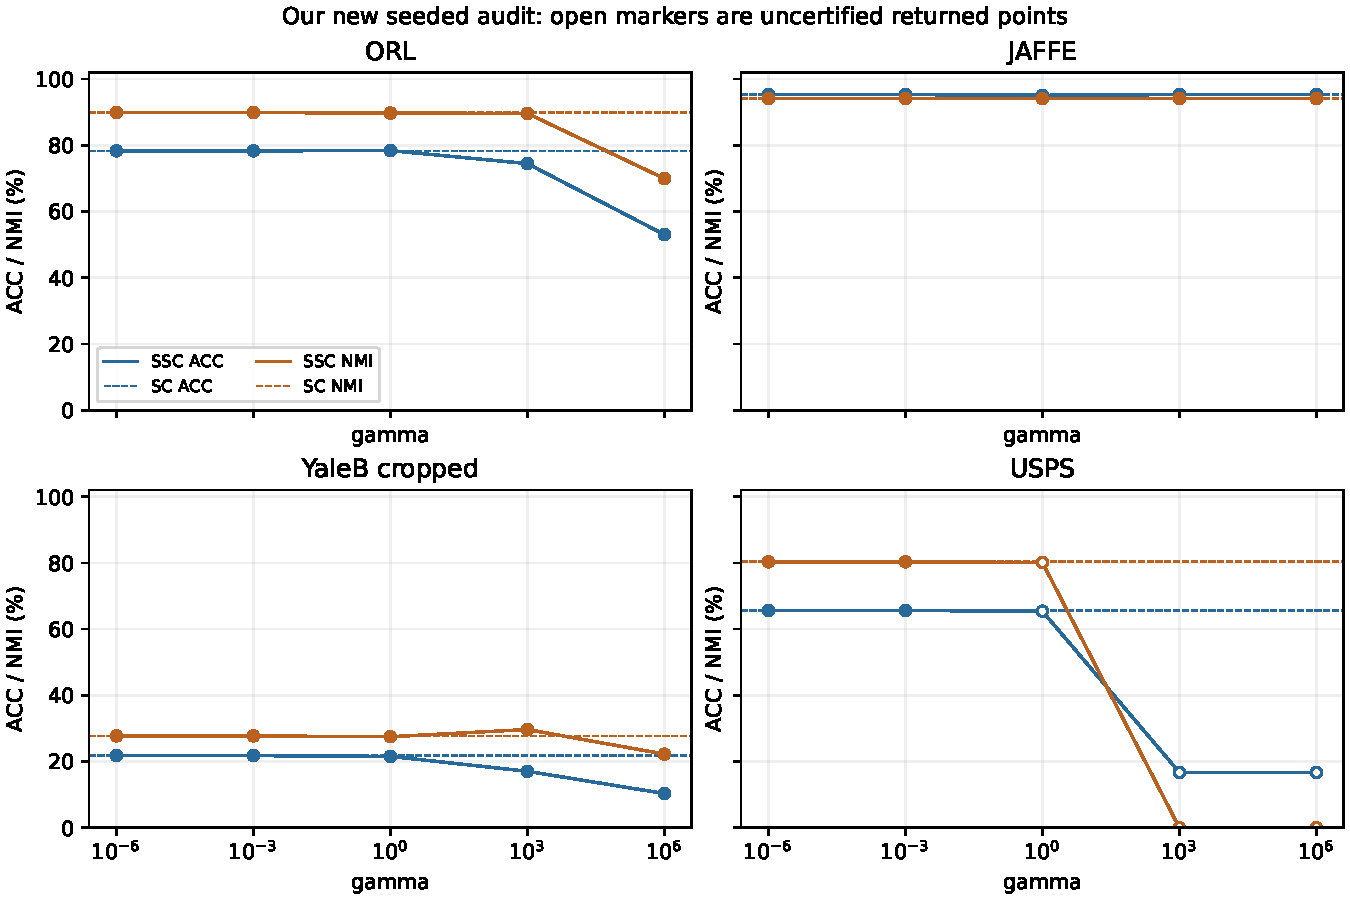
\includegraphics[width=\textwidth]{../results/next_round/figures/gamma_curves.pdf}\caption{Same seeded features and protocol; open markers are uncertified. These fresh points do not replace stronger historical points on unrecoverable old representations.}\end{figure}
\begin{figure}[h]\centering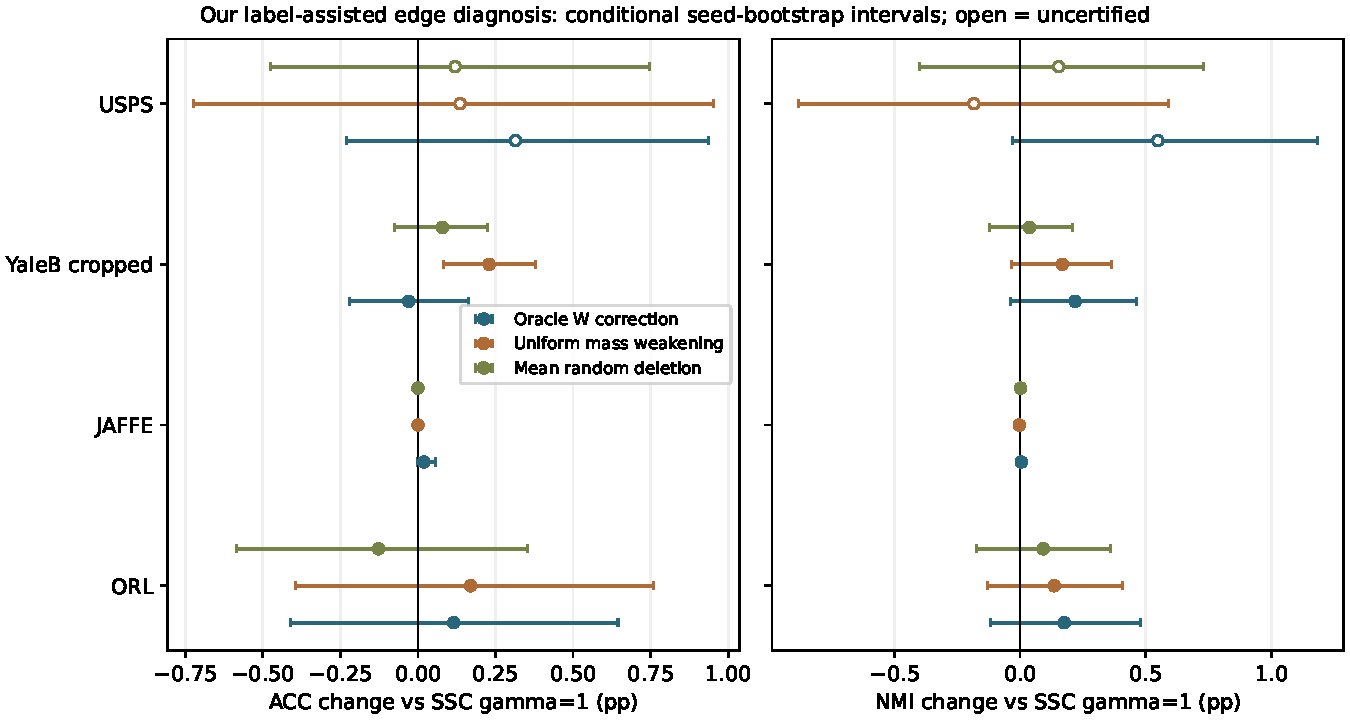
\includegraphics[width=\textwidth]{../results/next_round/figures/edge_diagnosis.pdf}\caption{Conditional paired seed intervals at gamma=1. Oracle correction is a label-assisted diagnostic, not an unsupervised method.}\end{figure}
\end{document}
